\documentclass{standalone}
\usepackage{tikz}
\usepackage{hsbcommon}
\begin{document}
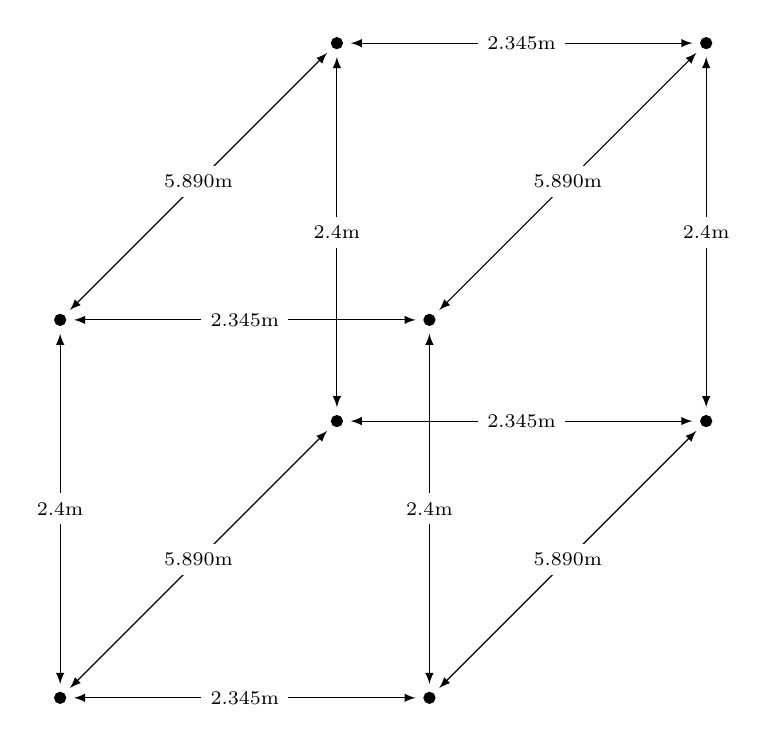
\begin{tikzpicture}[scale=2]
    %% inside dimensions
    
    \def\contheight{2.4}
    \def\contwidth{2.345}
    \def\contlength{5.890}
    \def\doorheight{2.29}
    \def\doorwidth{2.335}


    \tikzset{
        every path/.style={
            <->,>=latex, 
            shorten >=5pt, 
            shorten <=5pt
            },
        every node/.style={
            fill=white,
            font=\scriptsize
            }
        }

\foreach [count=\i] \ebene in {0,50}
{  
    \begin{scope}[xshift=\ebene,yshift=\ebene]
        
        \coordinate (A\i 1) at (0,0);
        \coordinate (A\i 2) at (\contwidth,0);
        \coordinate (A\i 3) at (\contwidth,\contheight);
        \coordinate (A\i 4) at (0,\contheight);
    
        \foreach \punkt in {1,2,3,4}
            \filldraw (A\i \punkt) circle (1pt);
    
        \draw (A\i 1) -- node {\contwidth m} (A\i 2) ;
        \draw (A\i 2) -- node  {\contheight m} (A\i 3) ;
        \draw (A\i 3) -- node {\contwidth m} (A\i 4) ;
        \draw (A\i 4) -- node  {\contheight m} (A\i 1) ;
    
    \end{scope}
}

        \foreach \punkt in {1,2,3,4}
            \draw (A1\punkt) -- node  {\contlength m} (A2\punkt); 


\end{tikzpicture}
\end{document}